\documentclass[12pt]{article}

%packages
%\usepackage{latexsym}
\usepackage{graphicx}
\usepackage{color}
\usepackage{amsmath}
\usepackage{dsfont}
\usepackage{placeins}
\usepackage{amssymb}
\usepackage{wasysym}
\usepackage{abstract}
\usepackage{hyperref}
\usepackage{etoolbox}
\usepackage{datetime}
\usepackage{xcolor}
\usepackage{alphalph}
\settimeformat{ampmtime}

%\usepackage{pstricks,pst-node,pst-tree}

%\usepackage{algpseudocode}
%\usepackage{amsthm}
%\usepackage{hyperref}
%\usepackage{mathrsfs}
%\usepackage{amsfonts}
%\usepackage{bbding}
%\usepackage{listings}
%\usepackage{appendix}
\usepackage[margin=1in]{geometry}
%\geometry{papersize={8.5in,11in},total={6.5in,9in}}
%\usepackage{cancel}
%\usepackage{algorithmic, algorithm}

\makeatletter
\def\maxwidth{ %
  \ifdim\Gin@nat@width>\linewidth
    \linewidth
  \else
    \Gin@nat@width
  \fi
}
\makeatother

\definecolor{fgcolor}{rgb}{0.345, 0.345, 0.345}
\newcommand{\hlnum}[1]{\textcolor[rgb]{0.686,0.059,0.569}{#1}}%
\newcommand{\hlstr}[1]{\textcolor[rgb]{0.192,0.494,0.8}{#1}}%
\newcommand{\hlcom}[1]{\textcolor[rgb]{0.678,0.584,0.686}{\textit{#1}}}%
\newcommand{\hlopt}[1]{\textcolor[rgb]{0,0,0}{#1}}%
\newcommand{\hlstd}[1]{\textcolor[rgb]{0.345,0.345,0.345}{#1}}%
\newcommand{\hlkwa}[1]{\textcolor[rgb]{0.161,0.373,0.58}{\textbf{#1}}}%
\newcommand{\hlkwb}[1]{\textcolor[rgb]{0.69,0.353,0.396}{#1}}%
\newcommand{\hlkwc}[1]{\textcolor[rgb]{0.333,0.667,0.333}{#1}}%
\newcommand{\hlkwd}[1]{\textcolor[rgb]{0.737,0.353,0.396}{\textbf{#1}}}%

\usepackage{framed}
\makeatletter
\newenvironment{kframe}{%
 \def\at@end@of@kframe{}%
 \ifinner\ifhmode%
  \def\at@end@of@kframe{\end{minipage}}%
  \begin{minipage}{\columnwidth}%
 \fi\fi%
 \def\FrameCommand##1{\hskip\@totalleftmargin \hskip-\fboxsep
 \colorbox{shadecolor}{##1}\hskip-\fboxsep
     % There is no \\@totalrightmargin, so:
     \hskip-\linewidth \hskip-\@totalleftmargin \hskip\columnwidth}%
 \MakeFramed {\advance\hsize-\width
   \@totalleftmargin\z@ \linewidth\hsize
   \@setminipage}}%
 {\par\unskip\endMakeFramed%
 \at@end@of@kframe}
\makeatother

\definecolor{shadecolor}{rgb}{.77, .77, .77}
\definecolor{messagecolor}{rgb}{0, 0, 0}
\definecolor{warningcolor}{rgb}{1, 0, 1}
\definecolor{errorcolor}{rgb}{1, 0, 0}
\newenvironment{knitrout}{}{} % an empty environment to be redefined in TeX

\usepackage{alltt}
\usepackage[T1]{fontenc}

\newcommand{\qu}[1]{``#1''}
\newcounter{probnum}
\setcounter{probnum}{1}

%create definition to allow local margin changes
\def\changemargin#1#2{\list{}{\rightmargin#2\leftmargin#1}\item[]}
\let\endchangemargin=\endlist 

%allow equations to span multiple pages
\allowdisplaybreaks

%define colors and color typesetting conveniences
\definecolor{gray}{rgb}{0.5,0.5,0.5}
\definecolor{black}{rgb}{0,0,0}
\definecolor{white}{rgb}{1,1,1}
\definecolor{blue}{rgb}{0.5,0.5,1}
\newcommand{\inblue}[1]{\color{blue}#1 \color{black}}
\definecolor{green}{rgb}{0.133,0.545,0.133}
\newcommand{\ingreen}[1]{\color{green}#1 \color{black}}
\definecolor{yellow}{rgb}{1,1,0}
\newcommand{\inyellow}[1]{\color{yellow}#1 \color{black}}
\definecolor{orange}{rgb}{0.9,0.649,0}
\newcommand{\inorange}[1]{\color{orange}#1 \color{black}}
\definecolor{red}{rgb}{1,0.133,0.133}
\newcommand{\inred}[1]{\color{red}#1 \color{black}}
\definecolor{purple}{rgb}{0.58,0,0.827}
\newcommand{\inpurple}[1]{\color{purple}#1 \color{black}}
\definecolor{backgcode}{rgb}{0.97,0.97,0.8}
\definecolor{Brown}{cmyk}{0,0.81,1,0.60}
\definecolor{OliveGreen}{cmyk}{0.64,0,0.95,0.40}
\definecolor{CadetBlue}{cmyk}{0.62,0.57,0.23,0}

%define new math operators
\DeclareMathOperator*{\argmax}{arg\,max~}
\DeclareMathOperator*{\argmin}{arg\,min~}
\DeclareMathOperator*{\argsup}{arg\,sup~}
\DeclareMathOperator*{\arginf}{arg\,inf~}
\DeclareMathOperator*{\convolution}{\text{\Huge{$\ast$}}}
\newcommand{\infconv}[2]{\convolution^\infty_{#1 = 1} #2}
%true functions

%%%% GENERAL SHORTCUTS

%shortcuts for pure typesetting conveniences
\newcommand{\bv}[1]{\boldsymbol{#1}}

%shortcuts for compound constants
\newcommand{\BetaDistrConst}{\dfrac{\Gamma(\alpha + \beta)}{\Gamma(\alpha)\Gamma(\beta)}}
\newcommand{\NormDistrConst}{\dfrac{1}{\sqrt{2\pi\sigma^2}}}

%shortcuts for conventional symbols
\newcommand{\tsq}{\tau^2}
\newcommand{\tsqh}{\hat{\tau}^2}
\newcommand{\sigsq}{\sigma^2}
\newcommand{\sigsqsq}{\parens{\sigma^2}^2}
\newcommand{\sigsqovern}{\dfrac{\sigsq}{n}}
\newcommand{\tausq}{\tau^2}
\newcommand{\tausqalpha}{\tau^2_\alpha}
\newcommand{\tausqbeta}{\tau^2_\beta}
\newcommand{\tausqsigma}{\tau^2_\sigma}
\newcommand{\betasq}{\beta^2}
\newcommand{\sigsqvec}{\bv{\sigma}^2}
\newcommand{\sigsqhat}{\hat{\sigma}^2}
\newcommand{\sigsqhatmlebayes}{\sigsqhat_{\text{Bayes, MLE}}}
\newcommand{\sigsqhatmle}[1]{\sigsqhat_{#1, \text{MLE}}}
\newcommand{\bSigma}{\bv{\Sigma}}
\newcommand{\bSigmainv}{\bSigma^{-1}}
\newcommand{\thetavec}{\bv{\theta}}
\newcommand{\thetahat}{\hat{\theta}}
\newcommand{\thetahatmle}{\hat{\theta}_{\mathrm{MLE}}}
\newcommand{\thetavechatmle}{\hat{\thetavec}_{\mathrm{MLE}}}
\newcommand{\muhat}{\hat{\mu}}
\newcommand{\musq}{\mu^2}
\newcommand{\muvec}{\bv{\mu}}
\newcommand{\muhatmle}{\muhat_{\text{MLE}}}
\newcommand{\lambdahat}{\hat{\lambda}}
\newcommand{\lambdahatmle}{\lambdahat_{\text{MLE}}}
\newcommand{\etavec}{\bv{\eta}}
\newcommand{\alphavec}{\bv{\alpha}}
\newcommand{\minimaxdec}{\delta^*_{\mathrm{mm}}}
\newcommand{\ybar}{\bar{y}}
\newcommand{\xbar}{\bar{x}}
\newcommand{\Xbar}{\bar{X}}
\newcommand{\phat}{\hat{p}}
\newcommand{\Phat}{\hat{P}}
\newcommand{\Zbar}{\bar{Z}}
\newcommand{\iid}{~{\buildrel iid \over \sim}~}
\newcommand{\inddist}{~{\buildrel ind \over \sim}~}
\newcommand{\approxdist}{~{\buildrel approx \over \sim}~}
\newcommand{\equalsindist}{~{\buildrel d \over =}~}
\newcommand{\loglik}[1]{\ell\parens{#1}}
\newcommand{\thetahatkminone}{\thetahat^{(k-1)}}
\newcommand{\thetahatkplusone}{\thetahat^{(k+1)}}
\newcommand{\thetahatk}{\thetahat^{(k)}}
\newcommand{\half}{\frac{1}{2}}
\newcommand{\third}{\frac{1}{3}}
\newcommand{\twothirds}{\frac{2}{3}}
\newcommand{\fourth}{\frac{1}{4}}
\newcommand{\fifth}{\frac{1}{5}}
\newcommand{\sixth}{\frac{1}{6}}

%shortcuts for vector and matrix notation
\newcommand{\A}{\bv{A}}
\newcommand{\At}{\A^T}
\newcommand{\Ainv}{\inverse{\A}}
\newcommand{\B}{\bv{B}}
\newcommand{\K}{\bv{K}}
\newcommand{\Kt}{\K^T}
\newcommand{\Kinv}{\inverse{K}}
\newcommand{\Kinvt}{(\Kinv)^T}
\newcommand{\M}{\bv{M}}
\newcommand{\Bt}{\B^T}
\newcommand{\Q}{\bv{Q}}
\newcommand{\Qt}{\Q^T}
\newcommand{\R}{\bv{R}}
\newcommand{\Rt}{\R^T}
\newcommand{\Z}{\bv{Z}}
\newcommand{\X}{\bv{X}}
\newcommand{\Xsub}{\X_{\text{(sub)}}}
\newcommand{\Xsubadj}{\X_{\text{(sub,adj)}}}
\newcommand{\I}{\bv{I}}
\newcommand{\Y}{\bv{Y}}
\newcommand{\sigsqI}{\sigsq\I}
\renewcommand{\P}{\bv{P}}
\newcommand{\Psub}{\P_{\text{(sub)}}}
\newcommand{\Pt}{\P^T}
\newcommand{\Pii}{P_{ii}}
\newcommand{\Pij}{P_{ij}}
\newcommand{\IminP}{(\I-\P)}
\newcommand{\Xt}{\bv{X}^T}
\newcommand{\XtX}{\Xt\X}
\newcommand{\XtXinv}{\parens{\Xt\X}^{-1}}
\newcommand{\XtXinvXt}{\XtXinv\Xt}
\newcommand{\XXtXinvXt}{\X\XtXinvXt}
\newcommand{\x}{\bv{x}}
\renewcommand{\b}{\bv{b}}
\newcommand{\onevec}{\bv{1}}
\newcommand{\oneton}{1, \ldots, n}
\newcommand{\yoneton}{y_1, \ldots, y_n}
\newcommand{\yonetonorder}{y_{(1)}, \ldots, y_{(n)}}
\newcommand{\Yoneton}{Y_1, \ldots, Y_n}
\newcommand{\iinoneton}{i \in \braces{\oneton}}
\newcommand{\onetom}{1, \ldots, m}
\newcommand{\jinonetom}{j \in \braces{\onetom}}
\newcommand{\xoneton}{x_1, \ldots, x_n}
\newcommand{\Xoneton}{X_1, \ldots, X_n}
\newcommand{\xt}{\x^T}
\newcommand{\y}{\bv{y}}
\newcommand{\yt}{\y^T}
\renewcommand{\c}{\bv{c}}
\newcommand{\ct}{\c^T}
\newcommand{\tstar}{\bv{t}^*}
\renewcommand{\u}{\bv{u}}
\renewcommand{\v}{\bv{v}}
\renewcommand{\a}{\bv{a}}
\newcommand{\s}{\bv{s}}
\newcommand{\yadj}{\y_{\text{(adj)}}}
\newcommand{\xjadj}{\x_{j\text{(adj)}}}
\newcommand{\xjadjM}{\x_{j \perp M}}
\newcommand{\yhat}{\hat{\y}}
\newcommand{\yhatsub}{\yhat_{\text{(sub)}}}
\newcommand{\yhatstar}{\yhat^*}
\newcommand{\yhatstarnew}{\yhatstar_{\text{new}}}
\newcommand{\z}{\bv{z}}
\newcommand{\zt}{\z^T}
\newcommand{\bb}{\bv{b}}
\newcommand{\bbt}{\bb^T}
\newcommand{\bbeta}{\bv{\beta}}
\newcommand{\beps}{\bv{\epsilon}}
\newcommand{\bepst}{\beps^T}
\newcommand{\e}{\bv{e}}
\newcommand{\Mofy}{\M(\y)}
\newcommand{\KofAlpha}{K(\alpha)}
\newcommand{\ellset}{\mathcal{L}}
\newcommand{\oneminalph}{1-\alpha}
\newcommand{\SSE}{\text{SSE}}
\newcommand{\SSEsub}{\text{SSE}_{\text{(sub)}}}
\newcommand{\MSE}{\text{MSE}}
\newcommand{\RMSE}{\text{RMSE}}
\newcommand{\SSR}{\text{SSR}}
\newcommand{\SST}{\text{SST}}
\newcommand{\JSest}{\delta_{\text{JS}}(\x)}
\newcommand{\Bayesest}{\delta_{\text{Bayes}}(\x)}
\newcommand{\EmpBayesest}{\delta_{\text{EmpBayes}}(\x)}
\newcommand{\BLUPest}{\delta_{\text{BLUP}}}
\newcommand{\MLEest}[1]{\hat{#1}_{\text{MLE}}}

%shortcuts for Linear Algebra stuff (i.e. vectors and matrices)
\newcommand{\twovec}[2]{\bracks{\begin{array}{c} #1 \\ #2 \end{array}}}
\newcommand{\threevec}[3]{\bracks{\begin{array}{c} #1 \\ #2 \\ #3 \end{array}}}
\newcommand{\fivevec}[5]{\bracks{\begin{array}{c} #1 \\ #2 \\ #3 \\ #4 \\ #5 \end{array}}}
\newcommand{\twobytwomat}[4]{\bracks{\begin{array}{cc} #1 & #2 \\ #3 & #4 \end{array}}}
\newcommand{\threebytwomat}[6]{\bracks{\begin{array}{cc} #1 & #2 \\ #3 & #4 \\ #5 & #6 \end{array}}}

%shortcuts for conventional compound symbols
\newcommand{\thetainthetas}{\theta \in \Theta}
\newcommand{\reals}{\mathbb{R}}
\newcommand{\complexes}{\mathbb{C}}
\newcommand{\rationals}{\mathbb{Q}}
\newcommand{\integers}{\mathbb{Z}}
\newcommand{\naturals}{\mathbb{N}}
\newcommand{\forallninN}{~~\forall n \in \naturals}
\newcommand{\forallxinN}[1]{~~\forall #1 \in \reals}
\newcommand{\matrixdims}[2]{\in \reals^{\,#1 \times #2}}
\newcommand{\inRn}[1]{\in \reals^{\,#1}}
\newcommand{\mathimplies}{\quad\Rightarrow\quad}
\newcommand{\mathlogicequiv}{\quad\Leftrightarrow\quad}
\newcommand{\eqncomment}[1]{\quad \text{(#1)}}
\newcommand{\limitn}{\lim_{n \rightarrow \infty}}
\newcommand{\limitN}{\lim_{N \rightarrow \infty}}
\newcommand{\limitd}{\lim_{d \rightarrow \infty}}
\newcommand{\limitt}{\lim_{t \rightarrow \infty}}
\newcommand{\limitsupn}{\limsup_{n \rightarrow \infty}~}
\newcommand{\limitinfn}{\liminf_{n \rightarrow \infty}~}
\newcommand{\limitk}{\lim_{k \rightarrow \infty}}
\newcommand{\limsupn}{\limsup_{n \rightarrow \infty}}
\newcommand{\limsupk}{\limsup_{k \rightarrow \infty}}
\newcommand{\floor}[1]{\left\lfloor #1 \right\rfloor}
\newcommand{\ceil}[1]{\left\lceil #1 \right\rceil}

%shortcuts for environments
\newcommand{\beqn}{\vspace{-0.25cm}\begin{eqnarray*}}
\newcommand{\eeqn}{\end{eqnarray*}}
\newcommand{\bneqn}{\vspace{-0.25cm}\begin{eqnarray}}
\newcommand{\eneqn}{\end{eqnarray}}

%shortcuts for mini environments
\newcommand{\parens}[1]{\left(#1\right)}
\newcommand{\squared}[1]{\parens{#1}^2}
\newcommand{\tothepow}[2]{\parens{#1}^{#2}}
\newcommand{\prob}[1]{\mathbb{P}\parens{#1}}
\newcommand{\cprob}[2]{\prob{#1~|~#2}}
\newcommand{\littleo}[1]{o\parens{#1}}
\newcommand{\bigo}[1]{O\parens{#1}}
\newcommand{\Lp}[1]{\mathbb{L}^{#1}}
\renewcommand{\arcsin}[1]{\text{arcsin}\parens{#1}}
\newcommand{\prodonen}[2]{\bracks{\prod_{#1=1}^n #2}}
\newcommand{\mysum}[4]{\sum_{#1=#2}^{#3} #4}
\newcommand{\sumonen}[2]{\sum_{#1=1}^n #2}
\newcommand{\infsum}[2]{\sum_{#1=1}^\infty #2}
\newcommand{\infprod}[2]{\prod_{#1=1}^\infty #2}
\newcommand{\infunion}[2]{\bigcup_{#1=1}^\infty #2}
\newcommand{\infinter}[2]{\bigcap_{#1=1}^\infty #2}
\newcommand{\infintegral}[2]{\int^\infty_{-\infty} #2 ~\text{d}#1}
\newcommand{\supthetas}[1]{\sup_{\thetainthetas}\braces{#1}}
\newcommand{\bracks}[1]{\left[#1\right]}
\newcommand{\braces}[1]{\left\{#1\right\}}
\newcommand{\set}[1]{\left\{#1\right\}}
\newcommand{\abss}[1]{\left|#1\right|}
\newcommand{\norm}[1]{\left|\left|#1\right|\right|}
\newcommand{\normsq}[1]{\norm{#1}^2}
\newcommand{\inverse}[1]{\parens{#1}^{-1}}
\newcommand{\rowof}[2]{\parens{#1}_{#2\cdot}}

%shortcuts for functionals
\newcommand{\realcomp}[1]{\text{Re}\bracks{#1}}
\newcommand{\imagcomp}[1]{\text{Im}\bracks{#1}}
\newcommand{\range}[1]{\text{range}\bracks{#1}}
\newcommand{\colsp}[1]{\text{colsp}\bracks{#1}}
\newcommand{\rowsp}[1]{\text{rowsp}\bracks{#1}}
\newcommand{\tr}[1]{\text{tr}\bracks{#1}}
\newcommand{\rank}[1]{\text{rank}\bracks{#1}}
\newcommand{\proj}[2]{\text{Proj}_{#1}\bracks{#2}}
\newcommand{\projcolspX}[1]{\text{Proj}_{\colsp{\X}}\bracks{#1}}
\newcommand{\median}[1]{\text{median}\bracks{#1}}
\newcommand{\mean}[1]{\text{mean}\bracks{#1}}
\newcommand{\dime}[1]{\text{dim}\bracks{#1}}
\renewcommand{\det}[1]{\text{det}\bracks{#1}}
\newcommand{\expe}[1]{\mathbb{E}\bracks{#1}}
\newcommand{\expeabs}[1]{\expe{\abss{#1}}}
\newcommand{\expesub}[2]{\mathbb{E}_{#1}\bracks{#2}}
\newcommand{\indic}[1]{\mathds{1}_{#1}}
\newcommand{\var}[1]{\mathbb{V}\text{ar}\bracks{#1}}
\newcommand{\cov}[2]{\mathbb{C}\text{ov}\bracks{#1, #2}}
\newcommand{\corr}[2]{\text{Corr}\bracks{#1, #2}}
\newcommand{\se}[1]{\mathbb{S}\text{E}\bracks{#1}}
\newcommand{\seest}[1]{\hat{\mathbb{S}\text{E}}\bracks{#1}}
\newcommand{\bias}[1]{\text{Bias}\bracks{#1}}
\newcommand{\derivop}[2]{\dfrac{\text{d}}{\text{d} #1}\bracks{#2}}
\newcommand{\partialop}[2]{\dfrac{\partial}{\partial #1}\bracks{#2}}
\newcommand{\secpartialop}[2]{\dfrac{\partial^2}{\partial #1^2}\bracks{#2}}
\newcommand{\mixpartialop}[3]{\dfrac{\partial^2}{\partial #1 \partial #2}\bracks{#3}}

%shortcuts for functions
\renewcommand{\exp}[1]{\mathrm{exp}\parens{#1}}
\renewcommand{\cos}[1]{\text{cos}\parens{#1}}
\renewcommand{\sin}[1]{\text{sin}\parens{#1}}
\newcommand{\sign}[1]{\text{sign}\parens{#1}}
\newcommand{\are}[1]{\mathrm{ARE}\parens{#1}}
\newcommand{\natlog}[1]{\ln\parens{#1}}
\newcommand{\oneover}[1]{\frac{1}{#1}}
\newcommand{\overtwo}[1]{\frac{#1}{2}}
\newcommand{\overn}[1]{\frac{#1}{n}}
\newcommand{\oneoversqrt}[1]{\oneover{\sqrt{#1}}}
\newcommand{\sqd}[1]{\parens{#1}^2}
\newcommand{\loss}[1]{\ell\parens{\theta, #1}}
\newcommand{\losstwo}[2]{\ell\parens{#1, #2}}
\newcommand{\cf}{\phi(t)}

%English language specific shortcuts
\newcommand{\ie}{\textit{i.e.} }
\newcommand{\AKA}{\textit{AKA} }
\renewcommand{\iff}{\textit{iff}}
\newcommand{\eg}{\textit{e.g.} }
\newcommand{\st}{\textit{s.t.} }
\newcommand{\wrt}{\textit{w.r.t.} }
\newcommand{\mathst}{~~\text{\st}~~}
\newcommand{\mathand}{~~\text{and}~~}
\newcommand{\ala}{\textit{a la} }
\newcommand{\ppp}{posterior predictive p-value}
\newcommand{\dd}{dataset-to-dataset}

%shortcuts for distribution titles
\newcommand{\logistic}[2]{\mathrm{Logistic}\parens{#1,\,#2}}
\newcommand{\bernoulli}[1]{\mathrm{Bernoulli}\parens{#1}}
\newcommand{\betanot}[2]{\mathrm{Beta}\parens{#1,\,#2}}
\newcommand{\stdbetanot}{\betanot{\alpha}{\beta}}
\newcommand{\multnormnot}[3]{\mathcal{N}_{#1}\parens{#2,\,#3}}
\newcommand{\normnot}[2]{\mathcal{N}\parens{#1,\,#2}}
\newcommand{\classicnormnot}{\normnot{\mu}{\sigsq}}
\newcommand{\stdnormnot}{\normnot{0}{1}}
\newcommand{\uniformdiscrete}[1]{\mathrm{Uniform}\parens{\braces{#1}}}
\newcommand{\uniform}[2]{\mathrm{U}\parens{#1,\,#2}}
\newcommand{\stduniform}{\uniform{0}{1}}
\newcommand{\geometric}[1]{\mathrm{Geometric}\parens{#1}}
\newcommand{\hypergeometric}[3]{\mathrm{Hypergeometric}\parens{#1,\,#2,\,#3}}
\newcommand{\exponential}[1]{\mathrm{Exp}\parens{#1}}
\newcommand{\gammadist}[2]{\mathrm{Gamma}\parens{#1, #2}}
\newcommand{\poisson}[1]{\mathrm{Poisson}\parens{#1}}
\newcommand{\binomial}[2]{\mathrm{Binomial}\parens{#1,\,#2}}
\newcommand{\negbin}[2]{\mathrm{NegBin}\parens{#1,\,#2}}
\newcommand{\rayleigh}[1]{\mathrm{Rayleigh}\parens{#1}}
\newcommand{\multinomial}[2]{\mathrm{Multinomial}\parens{#1,\,#2}}
\newcommand{\gammanot}[2]{\mathrm{Gamma}\parens{#1,\,#2}}
\newcommand{\cauchynot}[2]{\text{Cauchy}\parens{#1,\,#2}}
\newcommand{\invchisqnot}[1]{\text{Inv}\chisq{#1}}
\newcommand{\invscaledchisqnot}[2]{\text{ScaledInv}\ncchisq{#1}{#2}}
\newcommand{\invgammanot}[2]{\text{InvGamma}\parens{#1,\,#2}}
\newcommand{\chisq}[1]{\chi^2_{#1}}
\newcommand{\ncchisq}[2]{\chi^2_{#1}\parens{#2}}
\newcommand{\ncF}[3]{F_{#1,#2}\parens{#3}}

%shortcuts for PDF's of common distributions
\newcommand{\logisticpdf}[3]{\oneover{#3}\dfrac{\exp{-\dfrac{#1 - #2}{#3}}}{\parens{1+\exp{-\dfrac{#1 - #2}{#3}}}^2}}
\newcommand{\betapdf}[3]{\dfrac{\Gamma(#2 + #3)}{\Gamma(#2)\Gamma(#3)}#1^{#2-1} (1-#1)^{#3-1}}
\newcommand{\normpdf}[3]{\frac{1}{\sqrt{2\pi#3}}\exp{-\frac{1}{2#3}(#1 - #2)^2}}
\newcommand{\normpdfvarone}[2]{\dfrac{1}{\sqrt{2\pi}}e^{-\half(#1 - #2)^2}}
\newcommand{\chisqpdf}[2]{\dfrac{1}{2^{#2/2}\Gamma(#2/2)}\; {#1}^{#2/2-1} e^{-#1/2}}
\newcommand{\invchisqpdf}[2]{\dfrac{2^{-\overtwo{#1}}}{\Gamma(#2/2)}\,{#1}^{-\overtwo{#2}-1}  e^{-\oneover{2 #1}}}
\newcommand{\exponentialpdf}[2]{#2\exp{-#2#1}}
\newcommand{\poissonpdf}[2]{\dfrac{e^{-#1} #1^{#2}}{#2!}}
\newcommand{\binomialpdf}[3]{\binom{#2}{#1}#3^{#1}(1-#3)^{#2-#1}}
\newcommand{\rayleighpdf}[2]{\dfrac{#1}{#2^2}\exp{-\dfrac{#1^2}{2 #2^2}}}
\newcommand{\gammapdf}[3]{\dfrac{#3^#2}{\Gamma\parens{#2}}#1^{#2-1}\exp{-#3 #1}}
\newcommand{\cauchypdf}[3]{\oneover{\pi} \dfrac{#3}{\parens{#1-#2}^2 + #3^2}}
\newcommand{\Gammaf}[1]{\Gamma\parens{#1}}

%shortcuts for miscellaneous typesetting conveniences
\newcommand{\notesref}[1]{\marginpar{\color{gray}\tt #1\color{black}}}

%%%% DOMAIN-SPECIFIC SHORTCUTS

%Real analysis related shortcuts
\newcommand{\zeroonecl}{\bracks{0,1}}
\newcommand{\forallepsgrzero}{\forall \epsilon > 0~~}
\newcommand{\lessthaneps}{< \epsilon}
\newcommand{\fraccomp}[1]{\text{frac}\bracks{#1}}

%Bayesian related shortcuts
\newcommand{\yrep}{y^{\text{rep}}}
\newcommand{\yrepisq}{(\yrep_i)^2}
\newcommand{\yrepvec}{\bv{y}^{\text{rep}}}


%Probability shortcuts
\newcommand{\SigField}{\mathcal{F}}
\newcommand{\ProbMap}{\mathcal{P}}
\newcommand{\probtrinity}{\parens{\Omega, \SigField, \ProbMap}}
\newcommand{\convp}{~{\buildrel p \over \rightarrow}~}
\newcommand{\convLp}[1]{~{\buildrel \Lp{#1} \over \rightarrow}~}
\newcommand{\nconvp}{~{\buildrel p \over \nrightarrow}~}
\newcommand{\convae}{~{\buildrel a.e. \over \longrightarrow}~}
\newcommand{\convau}{~{\buildrel a.u. \over \longrightarrow}~}
\newcommand{\nconvau}{~{\buildrel a.u. \over \nrightarrow}~}
\newcommand{\nconvae}{~{\buildrel a.e. \over \nrightarrow}~}
\newcommand{\convd}{~{\buildrel \mathcal{D} \over \rightarrow}~}
\newcommand{\nconvd}{~{\buildrel \mathcal{D} \over \nrightarrow}~}
\newcommand{\withprob}{~~\text{w.p.}~~}
\newcommand{\io}{~~\text{i.o.}}

\newcommand{\Acl}{\bar{A}}
\newcommand{\ENcl}{\bar{E}_N}
\newcommand{\diam}[1]{\text{diam}\parens{#1}}

\newcommand{\taua}{\tau_a}

\newcommand{\myint}[4]{\int_{#2}^{#3} #4 \,\text{d}#1}
\newcommand{\laplacet}[1]{\mathscr{L}\bracks{#1}}
\newcommand{\laplaceinvt}[1]{\mathscr{L}^{-1}\bracks{#1}}
\renewcommand{\min}[1]{\text{min}\braces{#1}}
\renewcommand{\max}[1]{\text{max}\braces{#1}}

\newcommand{\Vbar}[1]{\bar{V}\parens{#1}}
\newcommand{\expnegrtau}{\exp{-r\tau}}

%%% problem typesetting
\definecolor{darkgrey}{rgb}{0.10,0.10,0.9}

\newcommand{\problem}[1]{\noindent \colorbox{black}{{\color{yellow} \large{\textsf{\textbf{Problem \arabic{probnum}}}}~}} \addtocounter{probnum}{1} \vspace{0.2cm} \\ \iftoggle{professormode}{}{\color{darkgrey}} #1}

\newcommand{\easysubproblem}[1]{\ingreen{\item} \iftoggle{professormode}{}{\color{darkgrey}} [easy] #1 \color{black} }
\newcommand{\intermediatesubproblem}[1]{\inorange{\item} \iftoggle{professormode}{}{\color{darkgrey}} [harder] #1 \color{black} }
\newcommand{\hardsubproblem}[1]{\inred{\item} \iftoggle{professormode}{}{\color{darkgrey}} [difficult] #1 \color{black} }
\newcommand{\extracreditsubproblem}[1]{\inpurple{\item} \iftoggle{professormode}{}{\color{darkgrey}} [E.C.] #1 \color{black} }


\newcommand{\spc}[1]{\iftoggle{professormode}{\\ \vspace{#1cm}}{\\ \vspace{-0.3cm}}}

\makeatletter
\newalphalph{\alphmult}[mult]{\@alph}{26}
\renewcommand{\labelenumi}{(\alphmult{\value{enumi}})}

\newcommand{\support}[1]{\text{Supp}\bracks{#1}}
\newcommand{\mode}[1]{\text{Mode}\bracks{#1}}
\newcommand{\IQR}[1]{\text{IQR}\bracks{#1}}
\newcommand{\quantile}[2]{\text{Quantile}\bracks{#1,\,#2}}


\newtoggle{professormode}
% \toggletrue{professormode} %STUDENTS: DELETE or COMMENT this line



\title{MATH 342W / 650.4 Spring \the\year~Homework \#2}

\author{Mohammed Hasan} %STUDENTS: write your name here

\iftoggle{professormode}{
\date{Due 11:59PM Feb 25, \the\year \\ \vspace{0.5cm} \small (this document last updated \currenttime~on \today)}
}

\renewcommand{\abstractname}{Instructions and Philosophy}

\begin{document}
\maketitle

\iftoggle{professormode}{
\begin{abstract}
The path to success in this class is to do many problems. Unlike other courses, exclusively doing reading(s) will not help. Coming to lecture is akin to watching workout videos; thinking about and solving problems on your own is the actual ``working out.''  Feel free to \qu{work out} with others; \textbf{I want you to work on this in groups.}

Reading is still \textit{required}. You should be googling and reading about all the concepts introduced in class online. This is your responsibility to supplement in-class with your own readings.

The problems below are color coded: \ingreen{green} problems are considered \textit{easy} and marked \qu{[easy]}; \inorange{yellow} problems are considered \textit{intermediate} and marked \qu{[harder]}, \inred{red} problems are considered \textit{difficult} and marked \qu{[difficult]} and \inpurple{purple} problems are extra credit. The \textit{easy} problems are intended to be ``giveaways'' if you went to class. Do as much as you can of the others; I expect you to at least attempt the \textit{difficult} problems. 

This homework is worth 100 points but the point distribution will not be determined until after the due date. See syllabus for the policy on late homework.

Up to 7 points are given as a bonus if the homework is typed using \LaTeX. Links to instaling \LaTeX~and program for compiling \LaTeX~is found on the syllabus. You are encouraged to use \url{overleaf.com}. If you are handing in homework this way, read the comments in the code; there are two lines to comment out and you should replace my name with yours and write your section. The easiest way to use overleaf is to copy the raw text from hwxx.tex and preamble.tex into two new overleaf tex files with the same name. If you are asked to make drawings, you can take a picture of your handwritten drawing and insert them as figures or leave space using the \qu{$\backslash$vspace} command and draw them in after printing or attach them stapled.

The document is available with spaces for you to write your answers. If not using \LaTeX, print this document and write in your answers. I do not accept homeworks which are \textit{not} on this printout. Keep this first page printed for your records.

\end{abstract}

\thispagestyle{empty}
\vspace{1cm}
NAME: \line(1,0){380}
\clearpage
}

\problem{These are questions about Silver's book, chapter 2, 3.  Answer the questions using notation from class (i.e. $t ,f, g, h^*, \delta, \epsilon, e, t, z_1, \ldots, z_t, \mathbb{D}, \mathcal{H}, \mathcal{A}, \mathcal{X}, \mathcal{Y}, X, y, n, p, x_{\cdot 1}, \ldots, x_{\cdot p}, x_{1 \cdot}, \ldots, x_{n \cdot}$, etc).}


\begin{enumerate}

\intermediatesubproblem{If one's goal is to fit a model for a phenomenon $y$, what is the difference between the approaches of the hedgehog and the fox? Connecting this to the modeling framework should really make you think about what Tetlock's observation means for political and historical phenomena.}\spc{3}

The hedgehog's approach resembles more of a single, all-encompassing model \(h^*\) that relies heavily on a general principle, aiming to minimize error \(\epsilon\) through a complex model with many parameters \(\theta\). On the other hand, The fox's approach involves employing a variety of models \(\{g_1, g_2, ..., g_m\}\) that capture different aspects of the data \(D\) and phenomenon \(y\).

\easysubproblem{Why did Harry Truman like hedgehogs? Are there a lot of people that think this way?}\spc{2}

Harry Truman liked hedgehogs more because he wanted a “one-handed economist” meaning he wanted one straightforward answers rather than multiple conditional answers which foxes gave. Yes, many people think this way are considered part of a type A culture which contain industries like television, business, and politics.

\hardsubproblem{Why is it that the more education one acquires, the less accurate one's predictions become?}\spc{3}

"the more facts hedgehogs have at their command, the more opportunities they have to permute and manipulate them in ways that confirm their biases." This implies that when individuals with a hedgehog-like focus acquire more education and knowledge, their predictions can become less accurate due to an overconfidence in their own perspectives. This overconfidence leads them to manipulate information in ways that confirm their existing biases.

\easysubproblem{Why are probabilistic classifiers (i.e. algorithms that output functions that return probabilities) better than vanilla classifiers (i.e. algorithms that only return the class label)? We will move in this direction in class soon.}\spc{4}

Probabilistic classifiers show a range of possible outcomes rather than a single prediction which vanilla classifiers would show. 

\easysubproblem{What algorithm that we studied in class is PECOTA most similar to?}\spc{1}

PECOTA is most similar to KNN model, the K-nearest neighbors.

\easysubproblem{Is baseball performance as a function of age a linear model? Discuss.}\spc{4}

No. baseball performance as a function of age does not follow a linear model because age deterioration causes more of a bell curve with the higher points being the prime of a humans lifetime.

\intermediatesubproblem{How can baseball scouts do better than a prediction system like PECOTA?}\spc{6}

Baseball scouts can do better than a prediction system like PECOTA by looking into aspects of a player's performance and potential that are difficult to quantify through statistical analysis. PECOTA and other statistical models can analyze past performance data and compare players to other recorded players, scouts can assess intangible factors such as a player's work ethic, mental toughness, adaptability, and potential for growth beyond what their current statistics might suggest. Silver also experiences this first hand when he confronted Pedroia. "Pedroia
might have let the scouting reports go to his head and never have made the big leagues." which shows that the player had other factors such as mental toughness which allowed him to excel.

\intermediatesubproblem{Why hasn't anyone (at the time of the writing of Silver's book) taken advantage of Pitch f/x data to predict future success?}\spc{6}

"But someone will come along and take advantage of Pitch f/x data in a smart way, or will figure out how to fuse quantitative and qualitative evaluations of player performance." I believe this means that no one at the time had the abilities to evaluate players based on their quantitative and qualitative data. Which is why Pitch f/x wasnt being taken advantage of at the time.

\end{enumerate}



\problem{These are questions about the SVM.}

\begin{enumerate}

\easysubproblem{State the hypothesis set $\mathcal{H}$ inputted into the support vector machine algorithm. Is it different than the $\mathcal{H}$ used for $\mathcal{A}$ = perceptron learning algorithm?}\spc{1}

For the SVM algorithm, \(H\) consists of linear functions of the form \(h(x) = w \cdot x + b\), where \(w\) is the weight vector, \(b\) is the bias term, and \(x\) is the input feature vector. The entire point of the SVM is to find the optimal separating hyperplane that maximizes the margin between two classes in the feature space. On the other hand, for the Perceptron Learning Algorithm, the hypothesis set is also composed of linear functions \(h(x) = w \cdot x + b\). The difference being \(w\) and \(b\). The Perceptron Learning Algorithm updates its weights based on misclassified examples, without considering the margin between the classes. Meanwhile, the SVM explicitly maximizes this margin, which often results in a better generalization to unseen data.


\extracreditsubproblem{Prove the max-margin linearly separable SVM converges. State all assumptions. Write it on a separate page.}\spc{-0.5}

\hardsubproblem{Let $\mathcal{Y} = \braces{-1,1}$. Rederive the cost function whose minimization yields the SVM line in the linearly separable case. }\spc{20}

For a linearly separable case, the SVM's goal is to find a hyperplane that separates the classes with the maximum margin while correctly also satisying the dataset. The cost function's minimization gives us the SVM line that is based on maximizing the margin between the two classes, which is inversely proportional to the norm of the weight vector \(w\). In which case the problem is:

\[
\min{w, b} \frac{1}{2} \|w\|^2
\]

Where \(y_i \in \{-1, 1\}\) are the class labels, and \(x_i\) are the feature vectors of the training examples. 


\easysubproblem{Given your answer to (c) rederive the cost function using the \qu{soft margin} i.e. the hinge loss plus the term with the hyperparameter $\lambda$. This is marked easy since there is just one change from the expression given in class.}\spc{4}


\end{enumerate}



\problem{These are questions are about the $k$ nearest neighbors (KNN) algorithm.}

\begin{enumerate}

\easysubproblem{Describe how the algorithm works. Is $k$ a \qu{hyperparameter}?}\spc{5}

a predefined, k, is used to consider the nearest neighbors to consider for making a prediction. This k is a "hyperparameter," it is a parameter that is set before the learning process and directly influences the performance of the model.

\hardsubproblem{[MA] Assuming $\mathcal{A} = $ KNN, describe the input $\mathcal{H}$ as best as you can.}\spc{8}

\easysubproblem{When predicting on $\mathbb{D}$ with $k=1$, why should there be zero error? Is this a good estimate of future error when new data comes in? (Error in the future is called \emph{generalization error} and we will be discussing this later in the semester).}\spc{5}

The algorithm will select the closest point in the dataset to the query point and predict its value, this means there should be zero error because each point is its own neighbor as well. No, K=1 KNN model is is to constrained considering the dataset.

\end{enumerate}

\problem{These are questions about the linear model with $p=1$.}

\begin{enumerate}

\easysubproblem{What does $\mathbb{D}$ look like in the linear model with $p=1$? What is $\mathcal{X}$? What is $\mathcal{Y}$?}\spc{3}

The linear model p = 1 is a regular linear regression model that showcases a linear relationship between X and Y. This is when X is an independent prediction and Y is a dependant response.

\easysubproblem{Consider the line fit using the ordinary least squares (OLS) algorithm. Prove that the point $<\xbar, \ybar>$ is on this line. Use the formulas we derived in class.}\spc{3}

The equation for OLS is:

\[
y = \beta_0 + \beta_1 x
\]

where \(\beta_0\) is the y-intercept, and \(\beta_1\) is the slope of the line. 

\[
\beta_1 = \frac{\sum_{i=1}^{n} (x_i - \bar{x})(y_i - \bar{y})}{\sum_{i=1}^{n} (x_i - \bar{x})^2}
\]

\[
\beta_0 = \bar{y} - \beta_1 \bar{x}
\]

and to prove that $<\xbar, \ybar>$ is on this line, we can just sub in $\Bar{x}$ for x.

\intermediatesubproblem{Consider the line fit using OLS. Prove that the average prediction $\hat{y}_i := g(x_i)$ for $x_i \in \mathbb{D}$ is $\ybar$.}\spc{4}

The average prediction \(\hat{y}_i = g(x_i)\) for \(x_i \in D\) is \(\bar{y}\), we would use the simple linear regression model discussed earlier: \(g(x) = \hat{\beta}_0 + \hat{\beta}_1x\), where \(\hat{\beta}_0\) and \(\hat{\beta}_1\) are the OLS estimates for the intercept and slope. The average prediction over the dataset \(D\) is shown as:

\[
\frac{1}{n} \sum_{i=1}^{n} \hat{y}_i = \frac{1}{n} \sum_{i=1}^{n} (\hat{\beta}_0 + \hat{\beta}_1x_i)
\]

we can just isolate \(\hat{\beta}_0\) so that:

\[
\hat{\beta}_0 = \bar{y} - \hat{\beta}_1\bar{x}
\]

Substituting \(\hat{\beta}_0\) into our average prediction equation.


\intermediatesubproblem{Consider the line fit using OLS. Prove that the average residual $e_i$ is 0 over $\mathbb{D}$.}\spc{6}

The residual for each observation \(i\) is defined as \(e_i = y_i - \hat{y}_i\), where \(\hat{y}_i\) is the predicted value from our OLS model. The average residual over the dataset \(D\) is:

\[
\frac{1}{n} \sum_{i=1}^{n} e_i = \frac{1}{n} \sum_{i=1}^{n} (y_i - \hat{y}_i)
\]

By definition of the OLS, the sum and the average of residuals is zero, as the OLS minimizes the sum of squared residuals, \(SSR = \sum_{i=1}^{n} e_i^2\).


\intermediatesubproblem{Why is the RMSE usually a better indicator of predictive performance than $R^2$? Discuss in English.}\spc{4}

The RMSE and the coefficient of determination (\(R^2\)) both measure model performance, but RMSE is a better indicator of predictive performance because it directly quantifies the average error made by the model in the units of the outcome variable. RMSE is defined as:

\[
RMSE = \sqrt{\frac{1}{n} \sum_{i=1}^{n} (y_i - \hat{y}_i)^2}
\]

While \(R^2\) measures the proportion of the variance in the dependent variable that is predictable from the independent variables, it does not give information that the RMSE does.


\intermediatesubproblem{$R^2$ is commonly interpreted as \qu{proportion of the variance explained by the model} and proportions are constrained to the interval $\zeroonecl$. While it is true that $R^2 \leq 1$ for all models, it is not true that $R^2 \geq 0$ for all models. Construct an explicit example $\mathbb{D}$ and create a linear model $g(x) = w_0 + w_1 x$ whose $R^2 < 0$.}\spc{10}


\hardsubproblem{You are given $\mathbb{D}$ with $n$ training points $<x_i, y_i>$ but now you are also given a set of weights $\bracks{w_1~w_2~ \ldots ~w_n}$ which indicate how costly the error is for each of the $i$ points. Rederive the least squares estimates $b_0$ and $b_1$ under this situation. Note that these estimates are called the \emph{weighted least squares regression} estimates. This variant $\mathcal{A}$ on OLS has a number of practical uses, especially in Economics. No need to simplify your answers like I did in class (i.e. you can leave in ugly sums).}\spc{12.5}

Multi-variable linear regression used when you want $\vec{\hat{y}}$ to come close to $\vec{y}$. To do this we must use an intelligent weight $\vec{w}$. In the WLS model, each squared term in the loss function is weighted by a factor, which indicates how much weight or importance is given to that observation. $\vec{\hat{y}}$ are the predictions and $\vec{y}$ are the responses\\ 
$\hat{y} = 
\begin{pmatrix}
\hat{y}_1 \\
\vdots \\
\hat{y}_n
\end{pmatrix}$
= X $\vec{w}$ \\ 
$\vec{b} =$ argmin{SSE}

$\frac{\partial}{\partial \vec{w}}$ [SSE] =  ${\mathbf{\vec{0}}_{p+1}}$ \\
=> $\frac{\partial}{\partial \vec{w}}[\hat{y}^T\hat{y}-2w^T X^T \vec{y} + \vec{w}^T X^T X \vec{w}]$ \\
=> $\vec{\mathbf{0}_p+1}$ - 2$\frac{\partial}{\partial \vec{w}} [\vec{w}^T X^T \hat{y}$ + $\frac{\partial}{\partial \vec{w}} [\vec{w^T x^T X \vec{w}}]$ \\

where  $\vec{\mathbf{0}_p+1}$ satisfies Rule 0, - 2$\frac{\partial}{\partial \vec{w}} [\vec{w}^T X^T \hat{y}$ satisfies Rule 1, $\frac{\partial}{\partial \vec{w}} [\vec{w^T x^T X \vec{w}}]$ satisfies rule 3 and the unity satisfies rule 2.







\intermediatesubproblem{Interpret the ugly sums in the $b_0$ and $b_1$ you derived above and compare them to the $b_0$ and $b_1$ estimates in OLS. Does it make sense each term should be altered in this matter given your goal in the weighted least squares?}\spc{5}

In the standard OLS estimates, \(b_0\) and \(b_1\) are calculated without weighting the errors, which means all observations are ecaluated at an equal weight. This means that every observation contributes equally to the direction and position of the best-fit line, regardless of the reliability or importance of that observation. On the other hand, the WLS estimates adjust each term by the corresponding weight, \(w_i\), reflecting the proportionate importance of each observation.

%\hardsubproblem{[MA] In class we talked about $x_{raw} \in \braces{\text{red}, \text{green}}$ and the OLS model was the sample average of the inputted $x$ where $b_0 = \ybar_r$ and $b_1 = \ybar_g - \ybar_r$. Reparameterize $\mathcal{H} = \braces{w_1\indic{x_{raw} =~\text{red}}  + w_2 \indic{x_{raw} =~\text{green}}~:~ w_1, w_2 \in \reals}$ and prove that the OLS estimates are $b_1 = \ybar_r$ and $b_2 = \ybar_g$.}\spc{20}

\extracreditsubproblem{In class we talked about $x_{raw} \in \braces{\text{red}, \text{green}}$ and the OLS model was the sample average of the inputted $x$. Imagine if you have the additional constraint that $x_{raw}$ is ordinal e.g. $x_{raw} \in \braces{\text{low}, \text{high}}$ and you were forced to have a model where $g$(low) $\leq$ $g$(high). Write about an algorithm $\mathcal{A}$ that can solve this problem.}\spc{10}

\end{enumerate}

\problem{These are questions about association and correlation.}


\begin{enumerate}

\easysubproblem{Give an example of two variables that are both correlated and associated by drawing a plot.}\spc{7}

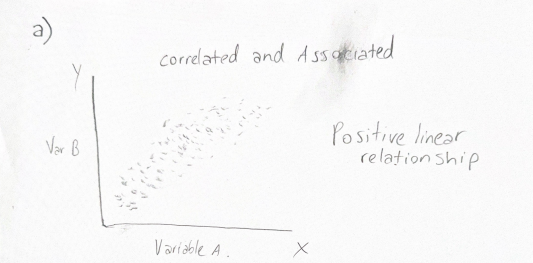
\includegraphics[scale=1]{Acorrelated.png}

\easysubproblem{Give an example of two variables that are not correlated but are associated by drawing a plot.}\spc{7}

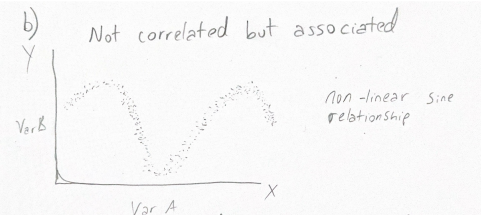
\includegraphics[scale=1]{Bcorrelated.png}

\easysubproblem{Give an example of two variables that are not correlated nor associated by drawing a plot.}\spc{7}\

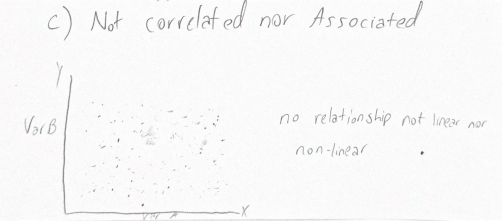
\includegraphics[scale=1]{Ccorrelated.png}

\easysubproblem{Can two variables be correlated but not associated? Explain.}\spc{7}

No, I believe correlation is a type of association and can't even visibly shown through a graph the possibility of "correlated but not associated"
\end{enumerate}


\problem{These are questions about multivariate linear model fitting using the least squares algorithm.}

\begin{enumerate}

\hardsubproblem{Derive $\partialop{\c}{\c^\top A \c}$ where $\c \in \reals^n$ and $A \in \reals^{n \times n}$ but \textit{not} symmetric. Get as far as you can.}\spc{8}

\easysubproblem{Given matrix $X \in \reals^{n \times (p+1)}$, full rank and first column consisting of the $\onevec_n$ vector, rederive the least squares solution $\b$ (the vector of coefficients in the linear model shipped in the prediction function $g$). No need to rederive the facts about vector derivatives.}\spc{10}

The least squares solution for the coefficients \(b\) in a linear model is derived from minimizing the sum of squared residuals. we can use the equation:
\[
b = (X^\top X)^{-1}X^\top y
\]



\intermediatesubproblem{Consider the case where $p = 1$. Show that the solution for $\b$ you just derived in (b) is the same solution that we proved for simple regression. That is, the first element of $\b$ is the same as $b_0 = \ybar - r \frac{s_y}{s_x}\xbar$ and the second element of $\b$ is $b_1 = r \frac{s_y}{s_x}$.} \spc{7}

When \(p = 1\), the matrix \(X\) consists of two columns: a column of ones (for the intercept) and a column for the single predictor variable. The solution derived in (b) simplifies to the formulas for \(b_0\) and \(b_1\) in simple linear regression:
\[
b_0 = \bar{y} - b_1\bar{x}
\]
\[
b_1 = \frac{r_{xy} s_y}{s_x}
\]
where \(r_{xy}\) is the correlation between \(x\) and \(y\), \(s_y\) and \(s_x\) are the standard deviations of \(y\) and \(x\) respectively, and \(\bar{y}\) and \(\bar{x}\) are the means of \(y\) and \(x\).


\easysubproblem{If $X$ is rank deficient, how can you solve for $\b$? Explain in English.} \spc{2}

When \(X\) is rank deficient, the matrix \(X^\top X\) is not invertible, which complicates finding a direct solution using the normal equation. we can add a term to the loss function, making \(X^\top X\) invertible by ensuring it is not rank deficient.


\hardsubproblem{Prove $\rank{X} =\rank{X^\top X}$.}\spc{9}

%\hardsubproblem{Given matrix $X \in \reals^{n \times (p+1)}$, full rank and first column consisting of the $\onevec_n$ vector, now consider cost multiples (\qu{weights}) $c_1, c_2, \ldots, c_n$ for each mistake $e_i$. As an example, previously the mistake for the 17th observation was $e_{17} := y_{17} - \hat{y}_{17}$ but now it would be $e_{17} := c_{17} (y_{17} - \hat{y}_{17})$.  Derive the weighted least squares solution $\b$. No need to rederive the facts about vector derivatives. Hints: (1) show that SSE is a quadratic form with the matrix $C$ in the middle (2) Split this matrix up into two pieces i.e. $C = C^{\half} C^{\half}$, distribute and then foil (3) note that a scalar value equals its own transpose and (4) use the vector derivative formulas.}\spc{10}


\intermediatesubproblem{[MA] If $p=1$, prove $r^2 = R^2$ i.e. the linear correlation is the same as proportion of sample variance explained in a least squares linear model.}\spc{6}

\intermediatesubproblem{Prove that $g(\bracks{1 ~\xbar_1~ \xbar_2~ \ldots~ \xbar_p}) =\bar{y}$ in OLS.}\spc{7}

\intermediatesubproblem{Prove that $\bar{e} = 0$ in OLS.}\spc{10}

\hardsubproblem{If you model $\y$ with one categorical nominal variable that has levels $A, B, C$, prove that the OLS estimates look like $\ybar_A$ if $x = A$, $\ybar_B$ if $x = B$ and $\ybar_C$ if $x = C$. You can choose to use an intercept or not. Likely without is easier.}\spc{10}


\intermediatesubproblem{[MA] Prove that the OLS model always has $R^2 \in \zeroonecl$.}\spc{5}

\end{enumerate}



\end{document}

